\chapter{Markov Blankets}\label{ch-mblanket}


This chapter is based on the
Wikipedia article, 
Ref.\cite{wiki-mblanket}.
Markov blankets
and Markov boundaries of bnets
were apparently invented
by Judea Pearl. His 1988 book
 Ref.\cite{pearl-1988book},
instead of a research paper, is 
usually given as the original reference.

\begin{figure}[h!]
\centering
\includegraphics[width=1.5in]{mblanket/mblanket.png}
\caption{In a bnet,
the minimal Markov blanket,
aka Markov boundary,
of node $\rva$.} 
\label{fig-mblanket}
\end{figure}

We will treat vectors 
of random variables as if
they were sets when using the $\in$,
$\subset$ and $-$ operations.
For example,
if $\rvx=(\rvx_0, 
\rvx_1, \rvx_2,
\rvx_3)$ and
$\rvb=(\rvx_1, \rvx_2)$,
then $\rvx_1\in \rvb\subset \rvx$ and
$\rvx-\rvb=(\rvx_0, \rvx_3)$.

Below, $H(\rva:\rvb|\rvc)$
denotes the conditional
mutual information of
random variables
$\rva$ and $\rvb$
conditioned on 
random variable $\rvc$.
$H(\rva:\rvb|\rvc)$
is used in Shannon Information
Theory, where it is defined by

\beq
H(\rva:\rvb|\rvc)=
\sum_{a,b,c}
P(a,b,c)\ln 
\frac{P(a,b|c)}{P(a|c)P(b|c)}
\;.
\eeq
$H(\rva:\rvb|\rvc)=0$
iff $\rva$ and $\rvb$
are independent (uncorrelated)
when $\rvc$ is held fixed.



Suppose
$\rva\in  \rvX$,
 $\rvB\subset \rvX$,
but $\rva\notin\rvB$.
Then $\rvB$ is a Markov blanket
of $\rva$ if

\beq
H(\rva: \rvX-\rva|\rvB)=0
\;.
\eeq
In other words, one may assume that
$\rva$ depends on $\rvB$ only, 
and is independent of all random
variables in $\rvX-(\rva\cup\rvB)$.

The minimal Markov blanket 
is called the Markov boundary.

In a bnet, the Markov boundary
of a node $\rva$,
contains:
\begin{enumerate}
\item
the parents of $\rva$,
\item
the children of $\rva$,
\item
the parents, other than $\rva$,
of the children of $\rva$.
\end{enumerate}
This is illustrated in 
Fig.\ref{fig-mblanket}.